\documentclass{sig-alternate-05-2015}
\usepackage[utf8]{inputenc}
\usepackage{graphicx}
\usepackage{csquotes}
\usepackage{hyperref}

\acmPrice{how did this get here i am not good with computer}

\begin{document}

\title{Network Cascades}
\subtitle{WattsApp With Those}
\author{Marco Brack \and Carsten Hartenfels}
\maketitle


\begin{abstract}
Concrete.
\end{abstract}


\section{Motivation}\label{sec:motivation}

Since caveman times people have been wondering how the ball gets rolling.

Communication technologies, such as Skype or WhatsApp, need users to actually be useful for communication between them. But how do these applications gain users in the first place then? They are mutually incompatible with each other, so surely if no one is using them, there is no reason for other people to start using them either.

One way to explain these phenomena is \emph{network cascades}. To stick with the high-level example above, assume that one person starts to use some communication technology. Then they tell their friends about it, convincing some of them to also begin using the application to communicate. Those friends to the same with their own friends, and so on and so forth. Given a suitably connected social network and a high enough ``convincability'' of its members, the usage will cascade through the entire network and eventually spread to all, or at least most, of its members. On the other hand, if the network does not have the required connectivity or if important bridge members cannot be convinced of the switch, the cascade may be halted and will not cause a global change in adoption.

% TODO: At least one more example

How to model these network cascades and what properties enable global cascades is the topic of the paper ``A simple model of global cascades on random networks'' by Duncan J. Watts\cite{simplemodel}. In this seminar paper, we will attempt to explain the contents of that paper in an effort to make the topic understandable to our fellow students.


\par\bigskip

Section \ref{sec:model} presents a simple network cascade model as laid out by Watts\cite{simplemodel}.

In section \ref{sec:example}, a walk-through of a simulation of a simple graph is given.


\section{Model}\label{sec:model}

The following section details Watts' simple model of network cascades\cite{simplemodel}. It explains the theoretical foundation and links it to the high-level example given in section \ref{sec:motivation}.

The model deals with a network of $n \in \mathbb{N}$ \emph{agents}. These agents are represented as nodes in a random graph. In regards to the example from section \ref{sec:motivation}, these agents represent people.

Relating this to the example, this might mean that Alice, Bob, Charly and Dave are ``agents'' who are faced with the decision if they should jump on the WhatsApp bandwagon and are thus each represented as a node in the network.

Each of these agents is connected to $k \in \mathbb{N}$ other nodes with a probability of $p_k \in [0,1]$. These edges represent the neighbors that each node observes, or in the example's terms, the person's friends. $p_k$ is poisson-distributed: $p_k = \frac{e^{-z}z^k}{k!}$, with $z = \left<k\right>$ being the expectation-value of $p_k$ (the average degree).

In our example, we choose $z$ to be 2. This means that the graph of the degree distribution for $p_k$ has its peak at 2 and that we would expect that most nodes have 2 neighbors. Plugging that into the distribution function tells us that the probability for this case (2 neighbors) is about $27\%$, and the probability for 1 neighbor is $27\%$, $18\%$ for 3 neighbors, $9\%$ for 4 and $3\%$ for 5, and so on. According to this, a ``realistic'' network for our potential WhatsApp users might have an connection between Alice and Bob, between Bob and Charly, and Charly and Dave, leaving Alice and Dave with each one neighbour, and Bob and Charly with each two neighbors. Figure \ref{fig:abcd} shows the graph for this setup.

\begin{figure}[h!]
    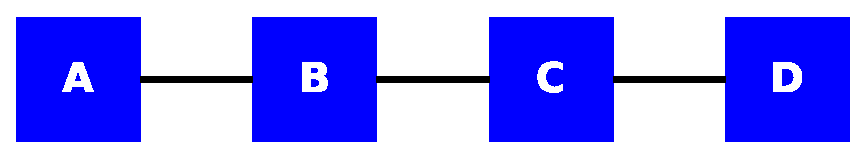
\includegraphics[width=\columnwidth]{img/abcd}
    \centering
    \caption{Alice, Bob, Charly and Dave}
    \label{fig:abcd}
\end{figure}

This random network model is equivalent to an Erdős–Rényi-Model with $p = \frac{z}{n}$. Networks following the Erdős–Rényi-Model are build by creating $n$ nodes and creating each possible edge with a probability $p$. This method generates networks which have a small average distances between nodes and a low amount of clustering.

In the example, there are $n = 4$ nodes. With $z = 2$ $p$ is $\frac{2}{4} = 0.5$, so we would expect half of all possible edges to exist. There are 6 possible edges in the network (this is excluding edges from a node to itself), and we chose to create 3, so our example indeed conforms perfectly to the Erdős–Rényi-Model.

Then each agent is given a threshold $\phi \in [0,1]$, drawn from an arbitrary random distribution $f(\phi): [0,1] \rightarrow [0,1]$ which must be normalized such that $\int_0^1 f(\phi) d\phi = 1$, i.e. the area beneath the probability function is 1, which means that all distributions must allocate the same total of probabilities. This restriction is necessary because we are assigning a probability to mutually exclusive ``events''. Relating to the example, this represents the ``convincability'' of a person.

The integral restriction is more easily understandable in a discrete case. For our WhatsApp example, we define the following discrete probability distribution:

$$
f(\phi) =
  \begin{cases}
    0 & \phi \in \{0, 1\} \\
    0.1 & \phi \in \{0.1, 0.2, 0.3, 0.4, 0.7, 0.8, 0.9\} \\
    0.2 & \phi \in \{0.5\}
  \end{cases}
$$

This means that the thresholds $0.1, 0.2, 0.3, 0.4, 0.7, 0.8, 0.9$ all have a probability of $10\%$ to be chosen, the threshold $0.5$ has a chance of $20\%$, and 0 and 1 will not be chosen at all. In contrast, we could assign a probability of $100\%$ to the threshold 0 and $0\%$ to all other thresholds and would still conform to the integral restriction.

Finally, all agents are given a state $\in \left\lbrace 0, 1 \right\rbrace$, which is initially set to $0$ for all notes. In the example's case, a state of $1$ represents a user of the communication application and a value of $0$ represents someone not using it.

Now the model is simulated over a time $t$, starting with $0$. At a random point in time, the state of a single node (the seed) is changed to $1$. This is analogous to the first person starting to use the application.

In independent random intervals, each node with state $0$ checks the state of all its neighbors. If the ratio of neighbors with states $1$ is greater than or equal to the node's threshold $\phi$, it will also change its state to $1$. This is the act of a person being ``convinced'' to begin using the application because enough of their friends are using it as well.

However, an agent with state $1$ will never switch back to state $0$. This does not directly map to a concept in a real-world example, as people may stop using an application at a later time. See also section \ref{sec:threats}.

In the example with Alice and the others, we apply the first probability distribution from above. Let us say that Alice and Bob are assigned a threshold of $\phi_{Alice} = \phi_{Bob} = 0.5$ (for which the probability is $20\%$), Charly is assigned $\phi_{Charly} = 0.3$ and Dave $\phi_{Dave} = 0.9$. This means that Dave is very hard to ``convince'', at least $90\%$ of his neighbors must use WhatsApp before he decides to use it (switch his state to $1$), whereas Charly already switches if only $30\%$ of his neighbors adopt the technology. Since Dave has only 1 neighbor, Charly, he switches as soon as Charly switches (in this case, $100\%$ of his neighbors would have switched). Dave has two neighbors, Bob and Dave, but only needs $30\%$ to switch, so it suffices if either Bob or Dave switch (that would be $50\%$ of his neighbors).

The model is then simulated over time until a steady state is reached. That is, the point where the entire system is stable and no agent will ever change its state again. The case of a steady state is easily verifiable: if all agents have observed their neighbors at least once since the last time any agent changed its state, then further observations will always lead to the same repeated result of no agent changing its state anymore. At this point, the simulation is finished.

After the simulation is done, there can be two results: either the experiment was successful and a global cascade has occurred, or the experiment has failed and the cascade was too small to be considered global.

What exactly constitutes as a successful global cascade is defined by $\frac{\textmd{Number of agents}}{\textmd{Agents in state } 1} \geq T$, where $T \in [0, 1]$ is some arbitrarily chosen threshold value. For example, $T = 1$ would require every last agent to have changed its state to $1$, which is difficult to achieve in a large random graph. A value like $T = 0.9$ would only require a 90\% majority, but still intuitively result in a cascade that was ``sufficiently global''.


\section{Example}\label{sec:example}

While the previous sections dealt with examples on an abstract level, this section walks through a detailed example of the actual model in action.

To keep the example from being overly long, we will use $n = 5$ agents. However, we have also built a simulation application\footnote{The application can be found at \url{https://github.com/turbopope/nss/tree/master/simulator}.}, which can be used to view examples in motion, with many more agents than we could fit into this paper.

Figure \ref{fig:model1} shows the initial state of the graph at $t = 0$. Each agent has its threshold set to a randomly chosen value and its state set to $0$.

\begin{figure}[h!]
    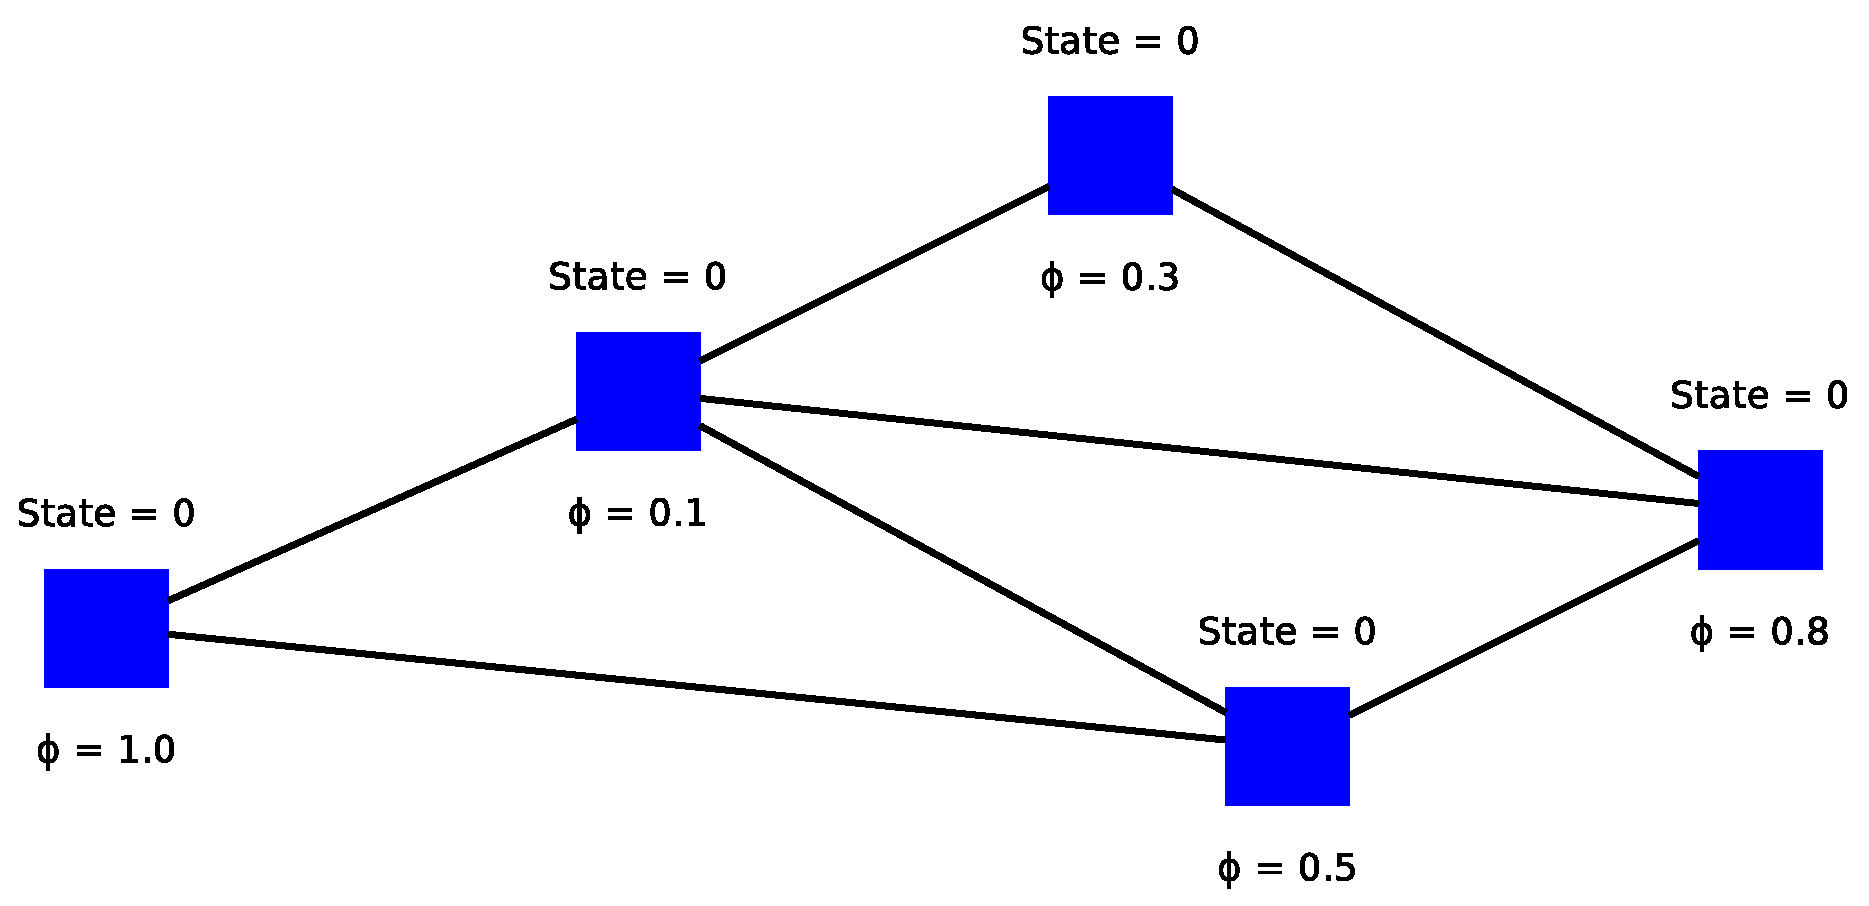
\includegraphics[width=\columnwidth]{../presentation/img/model4}
    \centering
    \caption{Initial State at $t = 0$}
    \label{fig:model1}
\end{figure}

In this configuration, nothing actually occurs yet however, since all states are $0$. All agents do periodically check their neighbors and calculate if they should change their own state, but of course this always results in no change. To actually begin the simulation proper, we must create the initial impulse. That is, we change the state of one node to $1$ at a random point in time. In this case, we have chosen the node with threshold $\phi = 1$. The new state can be seen in figure \ref{fig:model2}.

\begin{figure}[h!]
    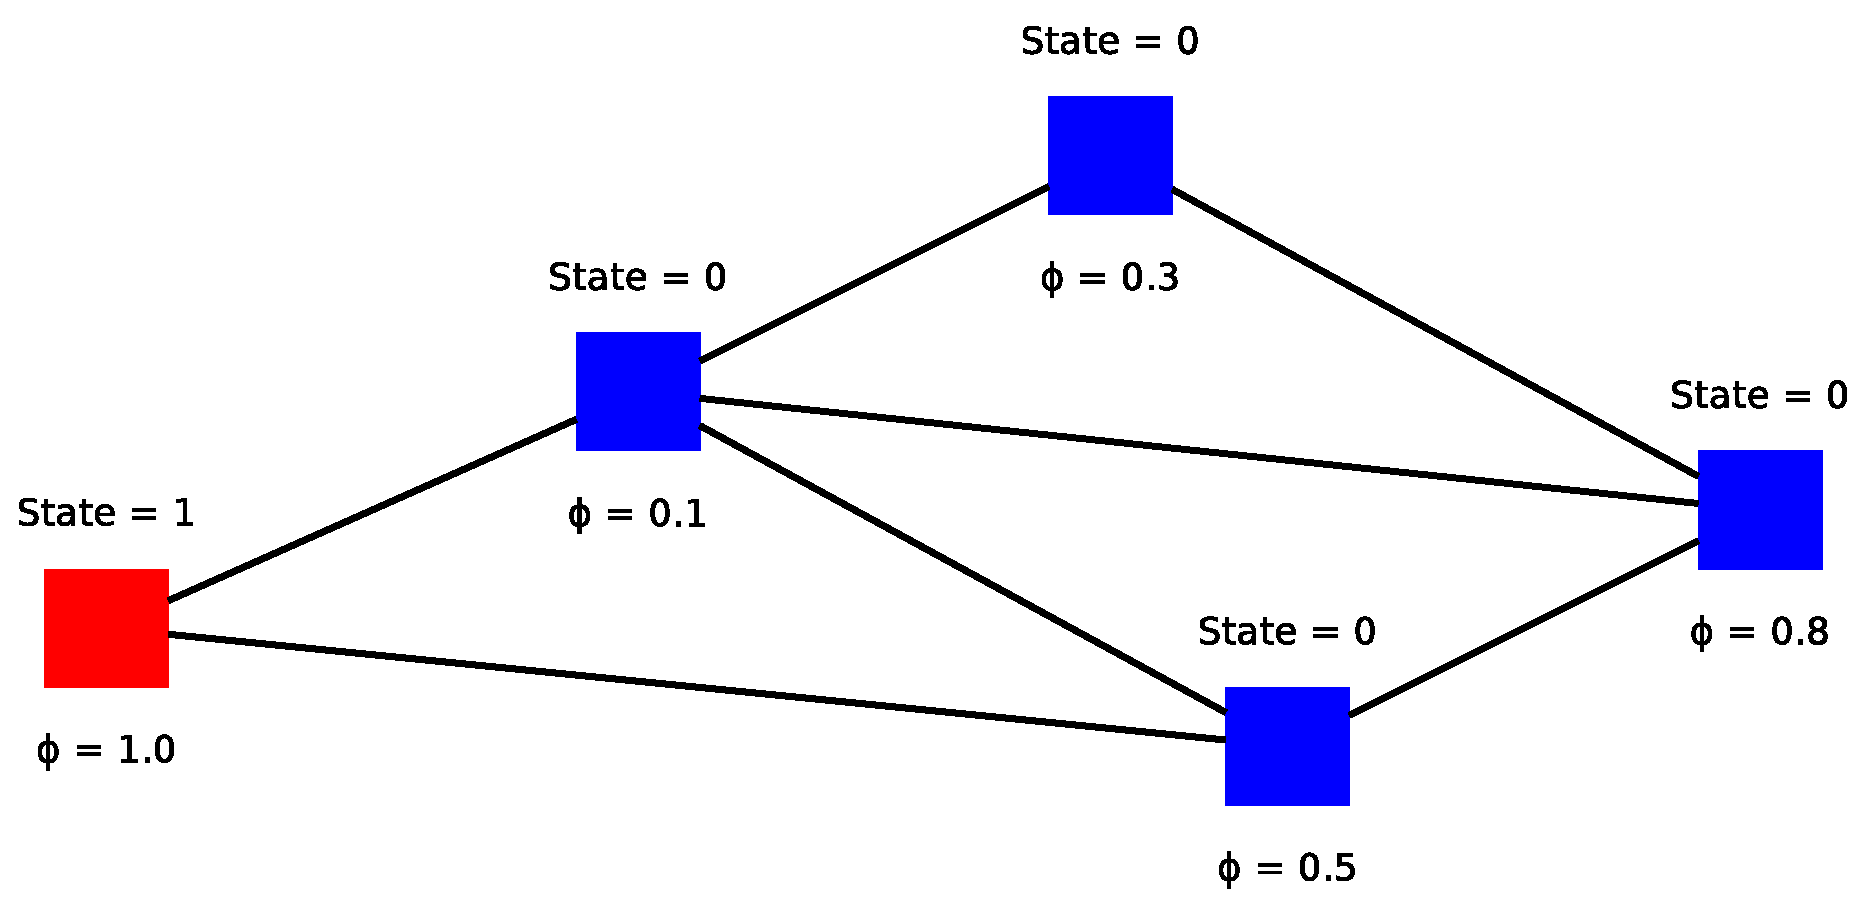
\includegraphics[width=\columnwidth]{../presentation/img/model5}
    \centering
    \caption{State after the initial impulse}
    \label{fig:model2}
\end{figure}

As the simulation keeps going, eventually the neighboring node with $\phi = 0.1$ will inspect its neighbors and notice the change. It has $4$ neighbors, of which $1$ is in state $1$. That means it compares $\frac{1}{4}$ to its own threshold of $0.1$. Since the calculated value is above the threshold, the node will change its own state to $1$. The new state of the network can be seen in figure \ref{fig:model3}.

\begin{figure}[h!]
    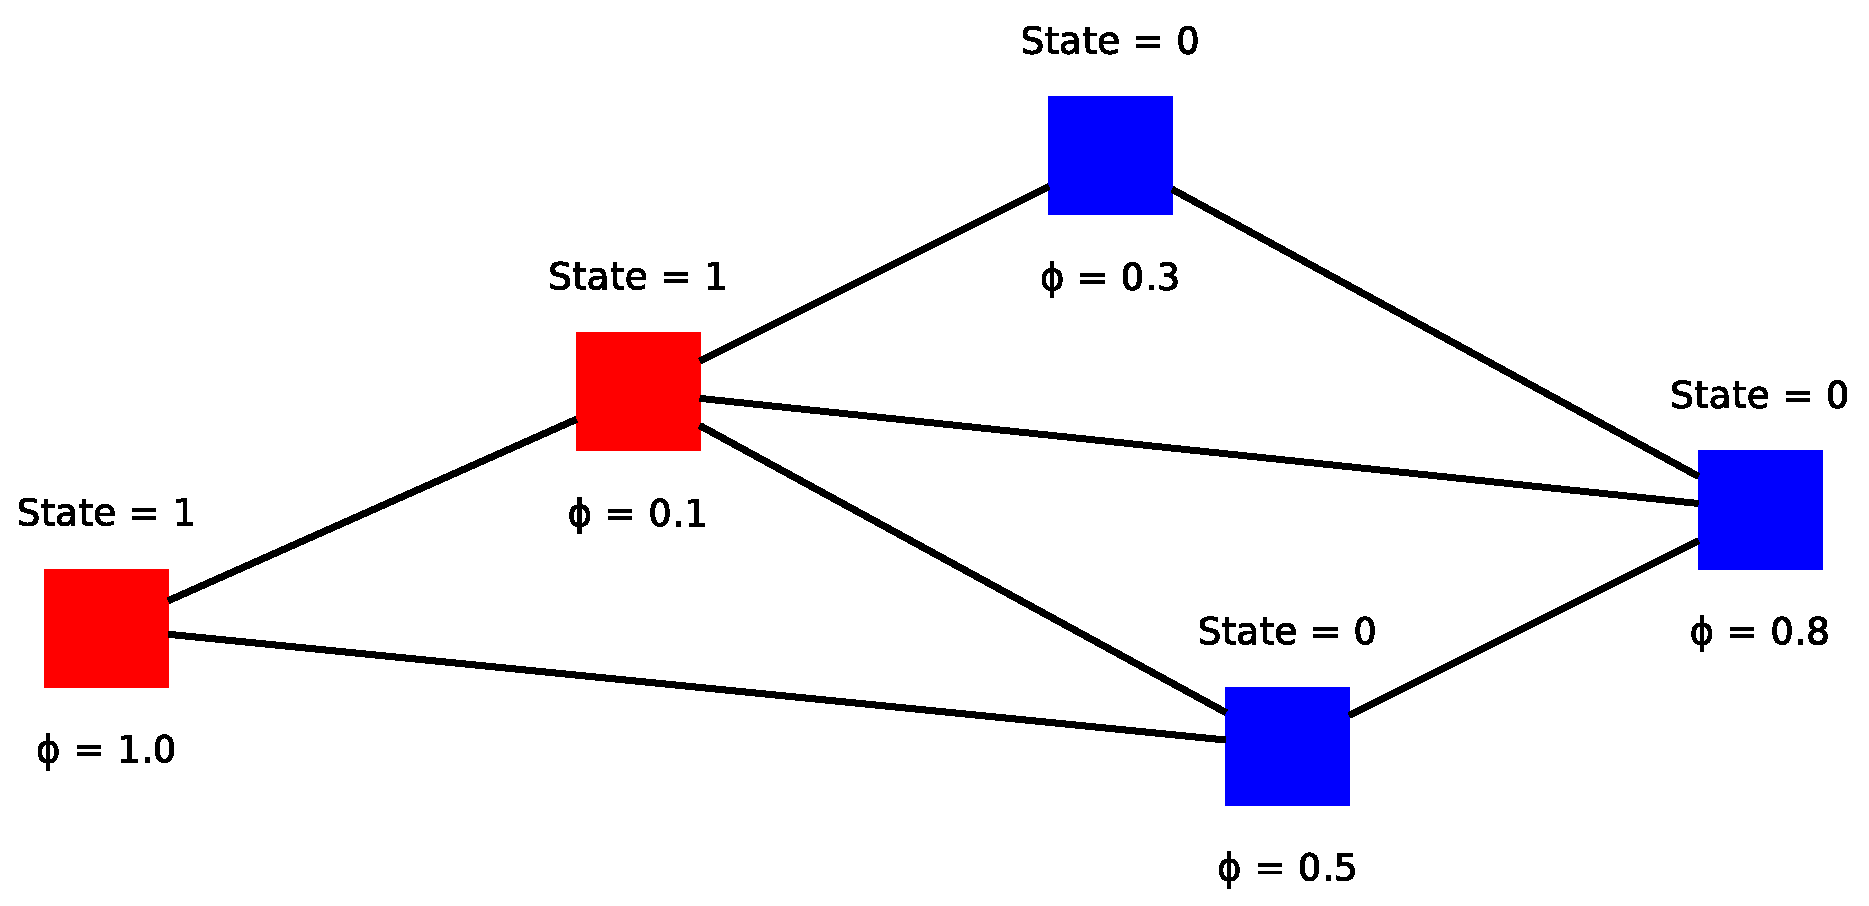
\includegraphics[width=\columnwidth]{../presentation/img/model6}
    \centering
    \caption{State after the second adoption}
    \label{fig:model3}
\end{figure}

There are also examples in which the state of the network does not change. For instance, if the node with threshold $\phi = 0.8$ checks its surroundings at this point, it will see that $1$ of its $3$ neighbors is in state $1$. However, since $\frac{1}{3}$ is below its own threshold of $0.8$, the node's state remains in state $0$.

Next, we will look at the node with threshold $\phi = 0.5$. It has $3$ neighbors, of which $2$ have already changed their state. Since $\frac{2}{3} > 0.5$, the node also changes its state and the graph's state looks like in figure \ref{fig:model4}.

\begin{figure}[h!]
    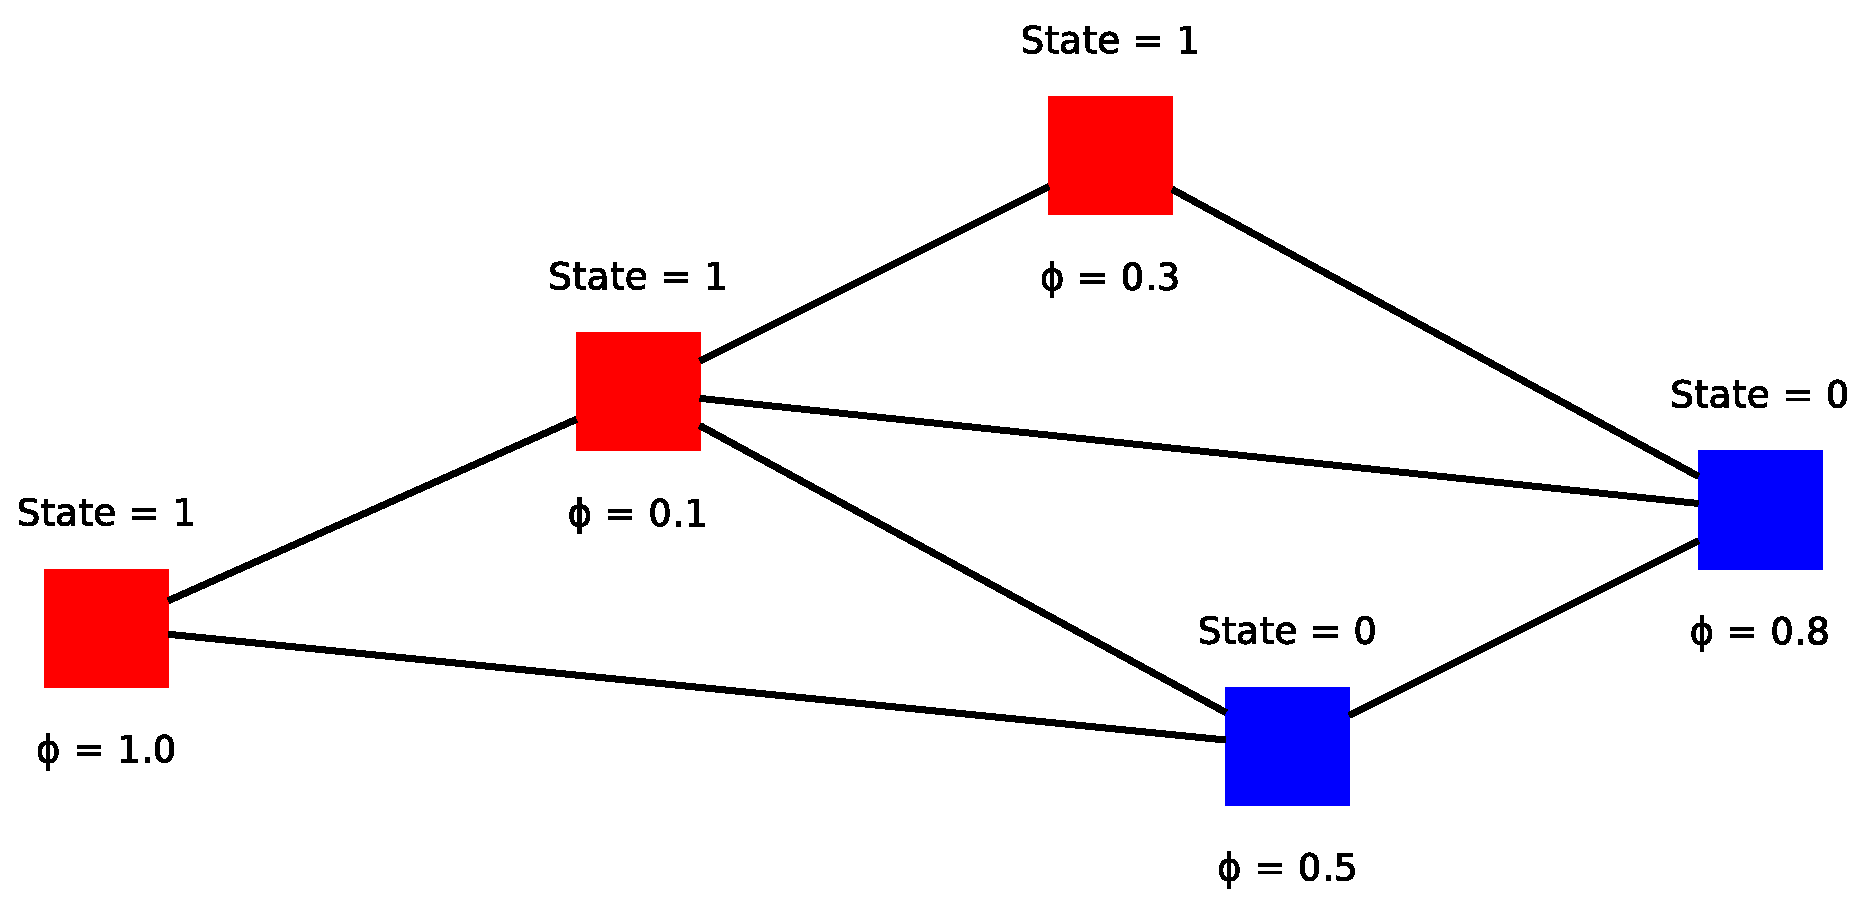
\includegraphics[width=\columnwidth]{../presentation/img/model7}
    \centering
    \caption{State after the third adoption}
    \label{fig:model4}
\end{figure}

As should be obvious by now, the final two nodes will also change their state at this point. First the node with $\phi = 0.5$ and finally the node with $\phi = 0.8$. At that point, the entire network is in a stable, unchanging state, as can be seen in figure \ref{fig:model5}. Since the entire network has changed its state to a uniform $1$, the cascade successfully worked its way from a single impulse to covering the entire network.

\begin{figure}[h!]
    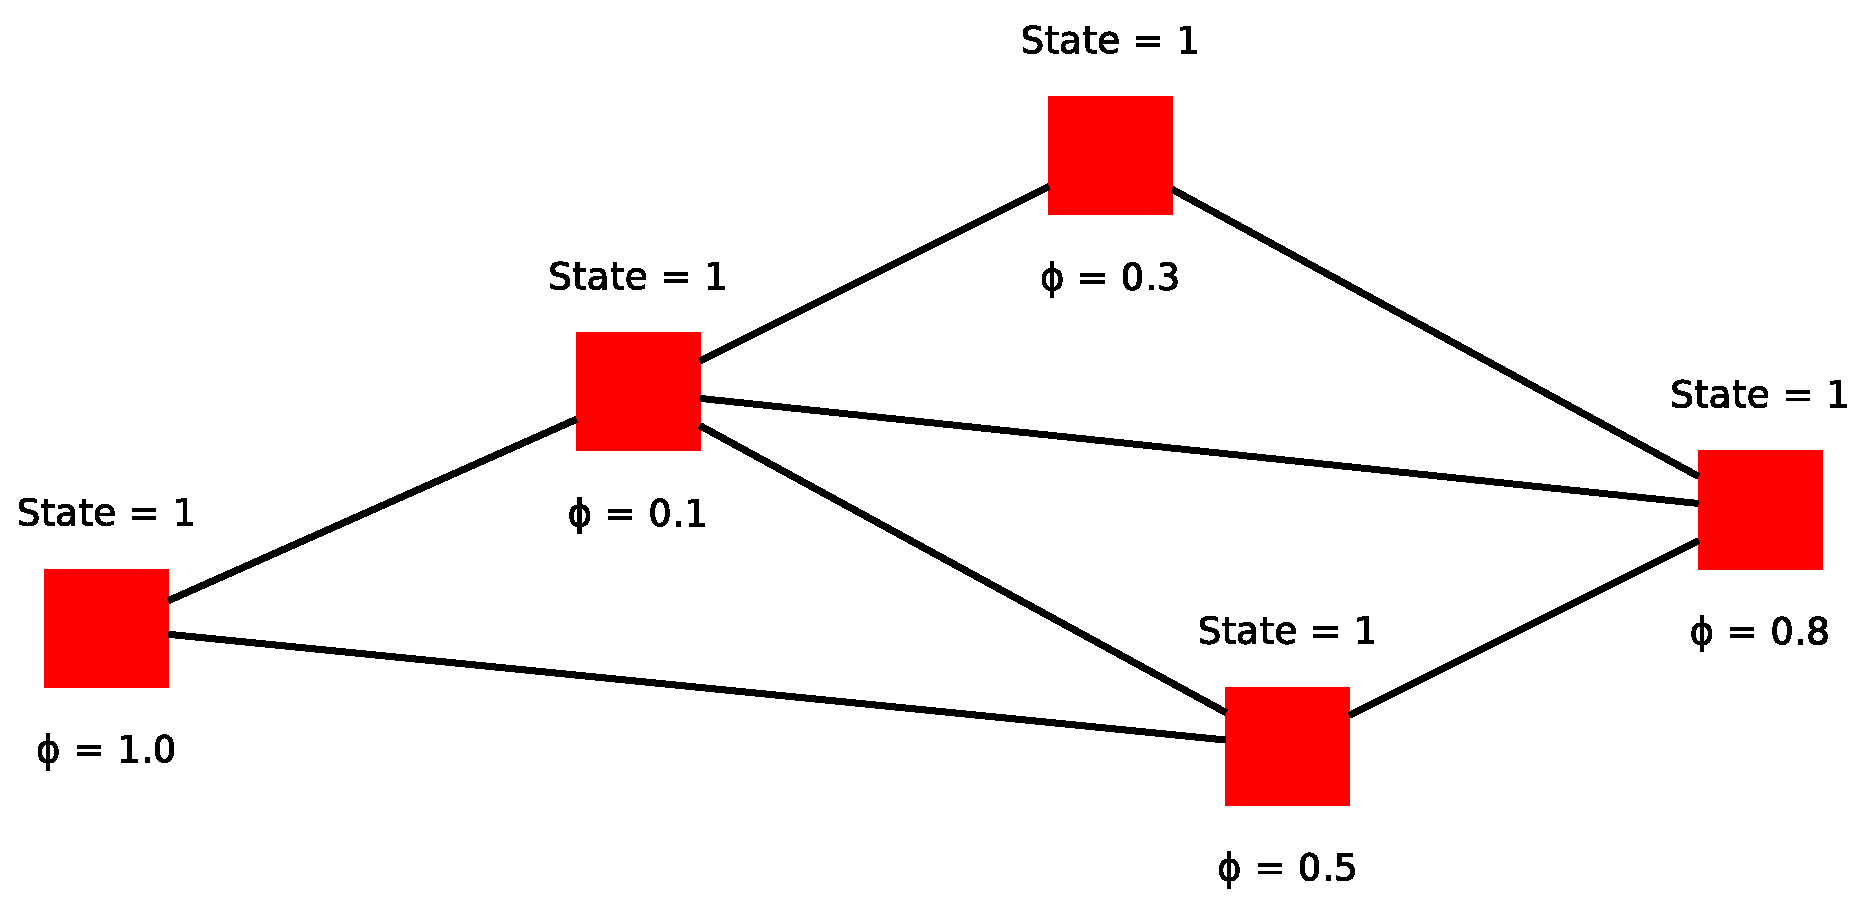
\includegraphics[width=\columnwidth]{../presentation/img/model9}
    \centering
    \caption{Final state -- successful cascade}
    \label{fig:model5}
\end{figure}

Different outcomes could have been possible as well, if a different node were chosen for the initial impulse. For instance, if the agent with $\phi = 0.1$ had been chosen, none of its neighbors would have had a low enough threshold to change their state at all. In that case, the system would have also entered a stable state, but the cascade would have failed to progress through the network.


\section{Cascade Condition}\label{sec:section}

Watts claims that global cascades are only possible if \textquote{the largest vulnerable cluster percolates}. This is called the \emph{cascade condition}.

That is, a successful cascade is only possible, if the graph's largest connected cluster of agents changes its state to $1$. This is only a necessary condition however: if the cascade condition is not fulfilled, a successful cascade is impossible, but a fulfilled cascade condition does not guarantee a successful cascade.

A node is vulnerable if its threshold is low enough so that only one of its neighbors needs to switch state for it to switch state itslef. Such nodes can be thought of as ``early adopters'' of a technology, with the initial seed beeing an ``innovator''. A vulerable cluster is a connected set of nodes that are ``early adopters'' (that are vulnerable) adjacent to an ``innovator''. This cluster must span a sufficiently (Watts never explicitly states what ``sufficient'' in this case means) large portion of the network (percolate) for the cascade condition to be true.

Through some generating functions black magic Watts expresses this cascade condition analytically. A cascade is possible if:

\begin{equation}
  G_0''(1) = \sum_{k=0}^\infty k (k-1) \rho_k p_k > z
\end{equation}

Let us break that down:

\begin{itemize}
  \item $\sum_{k=0}^\infty$: We iterate over all possible thresholds $k$ from $0$ to infinity. The sum converges and in reality it is possible to only calculate the ``first few'' elements
  \item $k (k-1)$ Nevermind that. These are remainders of the generating functions black magic.
  \item $\rho_k$ The probability that a node with degree k is vulerable (according to a probability distribution)
  \item $p_k$ The probability that a node has the threshold $k$ (according to a probability distribution)
\end{itemize}

In summary, for given probability distributions for both node degree and node threshold, the cascade condition inequation tells us if a vulnerable cluster percolates the network, meaning that global cascades are possible.

To illustrate this, let us choose those distributions and see what happens. We will construct a uniform graph with a homogenous threshold. Uniform graphs have a poisson degree distribution $p_k = \frac{e^{-z}z^k}{k!}$ with $z$ being the mean (the peak) of the distribution. The fixed threshold is easily modeled: The probability for a node being vulnerable is $\rho_k = P(\phi \leq \frac{1}{k})$, but since $\phi$ (the threshold) in this case is fixed, we just need to use $1$ for $\phi \leq \frac{1}{k}$ and $0$ for $\phi > \frac{1}{k}$ (and $1$ for $k = 0$).

For instance, let us see if cascades are possible for a fixed threshold $\phi = 0.2$ and a poisson-distributed degree with mean $z = 2$. Table \ref{tab:z2} shows the results for that graph.

\begin{table*}[t!]
\centering
\caption{Uniform graph with $\phi = 0.2$ and $z = 2$}
\label{tab:z2}
\begin{tabular}{|l|l|l|l|l|l|l|l|l|}
\hline
$k$                       & 0     & 1      & 2     & 3      & 4      & 5      & 6     & \ldots\\ \hline
$\rho_k$                  & 1     & 1      & 1     & 1      & 1      & 1      & 0     & \ldots\\ \hline
$p_k$                     & .135  & .271   & .271  & .18    & .09    & .036   & .012  & \ldots\\ \hline
$k (k-1) \rho_k p_k$      & 0     & 0      & .541  & 1.083  & 1.083  & 0.722  & 0     & \ldots\\ \hline
\end{tabular}
\end{table*}

The sum of the last row is $\sum_{k=0}^\infty k (k-1) \rho_k p_k = 3.428$, which is greater than $z = 2$, so cascades are possible in this case.

To put this in contrast, table \ref{tab:z8} examines the case of $\phi = 0.2$ and $z = 8$.

\begin{table*}
\centering
\caption{Uniform graph with $\phi = 0.2$ and $z = 8$}
\label{tab:z8}
\begin{tabular}{|l|l|l|l|l|l|l|l|l|}
\hline
$k$                       & 0  & 1     & 2     & 3     & 4     & 5      & 6     & \ldots\\ \hline
$\rho_k$                  & 1  & 1     & 1     & 1     & 1     & 1      & 0     & \ldots\\ \hline
$p_k$                     & 0  & .003  & .011  & .029  & .057  & .092   & .122  & \ldots\\ \hline
$k (k-1) \rho_k p_k$      & 0  & 0     & .021  & .172  & .687  & 1.832  & 0     & \ldots\\ \hline
\end{tabular}
\end{table*}

Here the sum of the last row is $\sum_{k=0}^\infty k (k-1) \rho_k p_k = 2.712$, which is smaller than $z = 8$, so no cascades will occur.

Watts tested this condition for these distributions for $z$ from $20$ to $0$ and $\phi$ from $0.1$ to $0.3$. Figure \ref{fig:cascade-window} depicts the results as a phase transition diagram (dashed line).

\begin{figure}[h!]
  \centering
  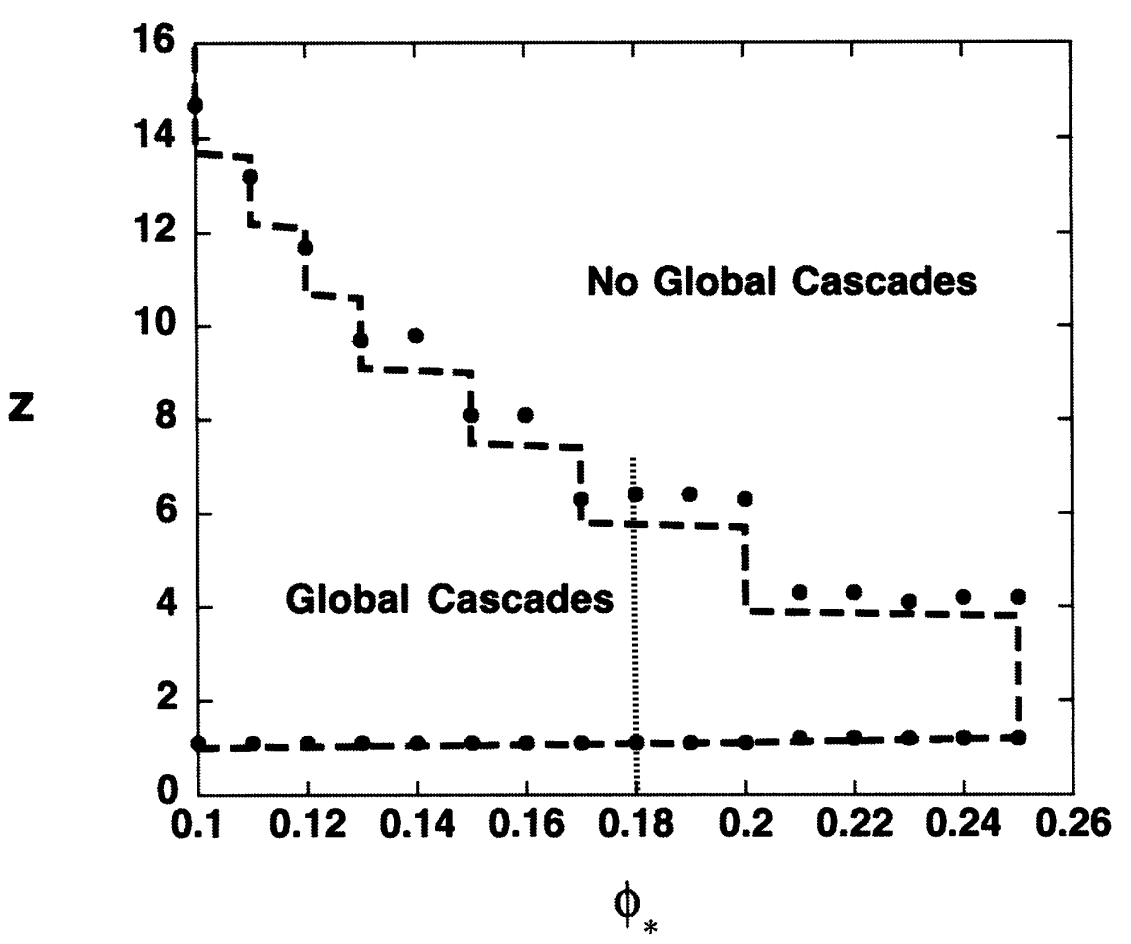
\includegraphics[width=0.45\textwidth]{img/cascade-regimes-with-cross-section.png}
  \caption{Cascade Window, image from \cite{simplemodel}}
  \label{fig:cascade-window}
\end{figure}

There are two areas in this diagram: One in which cascades are possible for the combination of $z$ and $\phi$ and one where no cascades are possible. It becomes apparent that there are two important transitions or ``boundaries'': One at an average degree $z = 1$ independent of the threshold, and one whith high average degrees and low threshold, with increasing threshold as the average degree decreases.

The dotted line in the diagram is the result of empirical testings where random networks where generated for the same distributions and the two parameters and tested, i.e. simulated. It is obvious that the calculated and the empirical phase transitions align (with reasonable precision), which validates the cascade condition inequation.

The cascade window diagram is limited to a binary statement wether cascades are possible. To gain further insight on the the nature of cascades inside the window, Watts examined ``cross section'' of the window for $\phi=0.18$ (marked in firgure \ref{fig:cascade-window} with by the densely stroked line at $\phi=0.18$), consisting of serveral measurements. They are depicted in figure \ref{fig:cross-section}. The upper graph (a) maps from $z$ to the amount of steps required for the cascade to occur. The lower figure (b) maps from $z$ to various percentages.

\begin{figure}[h!]
  \centering
  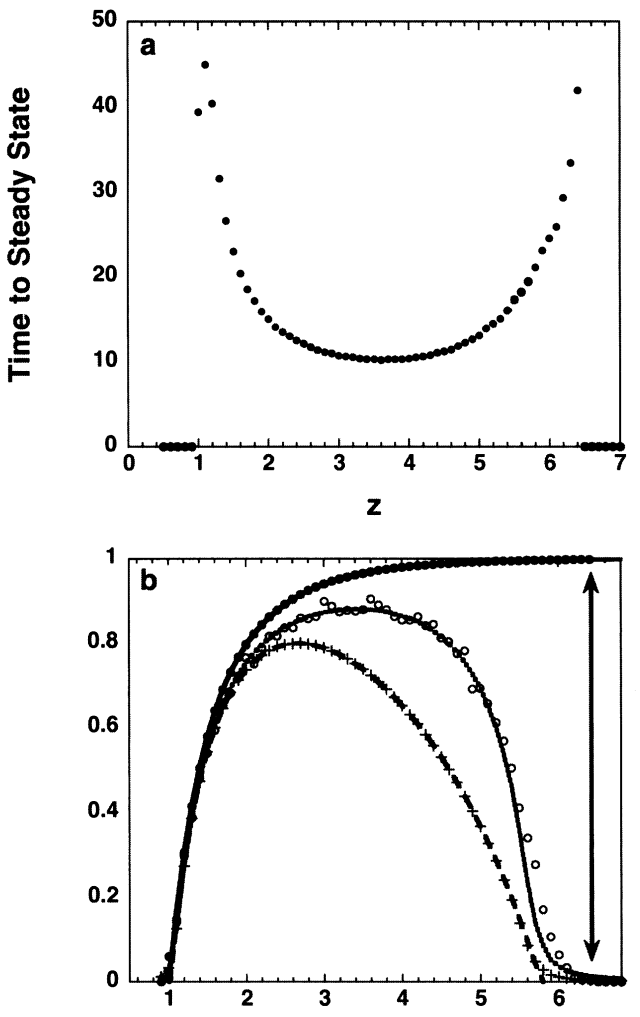
\includegraphics[width=0.45\textwidth]{img/cross-section.png}
  \caption{Cross section of the cascade window at $\phi=0.18$, image from \cite{simplemodel}}
  \label{fig:cross-section}
\end{figure}

There are 6 graphs here:

\begin{itemize}
  \item \textbf{Solid Circles \& Solid Line} -- These are optically very hard to distinguish from another, as they are virtually equal. They form the ``upper graph'' in the figure. The former shows the average size of global cascades and the latter shows the (analytical) size of the largest connected component, both as a fraction of the whole network.
  \item \textbf{Open Circles} -- Frequency of global cascades. Forms the ``middle graph''.
  \item \textbf{Short Dashes} -- Fractional (to the size of the network) size of the extended vulnerable cluster. The extended vulnerable cluster comprises the vulnerable cluster plus it's direct neighbors. Forms the ``middle graph''.
  \item \textbf{Long Dashes} -- The fractional (to the size of the network) size of the vulnerable cluster according to an analytical formula derived by Watts in the text. Forms the ``lower graph''.
  \item \textbf{Crosses} -- The fractional (to the size of the network) size of the vulnerable cluster, empirically determined by simulation. Forms the ``lower graph''.
\end{itemize}

Refer to section \ref{sec:findings} for Watts' interpretation of these graphs.

Further insights on the cascade window can be gained by examining the size of cascades around its boundaries. Figure \ref{fig:cascade-size} shows the cumulative distribution of the cascade sizes. The size of a cascade is measured in terms of the ratio between agents in state $1$ to the total number of agents. The examinded section of the window is the same as in figure \ref{fig:cross-section}. See \ref{sec:findings} for Watts' interpretation of this graph.


\section{Findings}\label{sec:findings}

In the above section \ref{fig:cross-section} was introduced as a means to compare the properties of the cascade window for a given threshold. Watts' interpretation of the results is as follows:

There is an obvious relation of the frequency of global cascades (open circles, in the middle) to the relative size of the vulnerable cluster (long dashes and crosses, the lower two graphs). They are roughly proportional, but the size of the cluster ``underestimates'' the cascade frequency. The given explanation for this is, that agents directly adjacent do the vulnerable cluster (who are themselves not vulnerable) can still trigger further cascades or promote the expansion of a cascade in the latter state of the cascade when most of it's vulnerable neighbors have been switched. This explanation is validated by examining the size of the extended vulnerable cluster, which comprises the vulnerable cluster plus its immediate (stable) neighbor nodes. And indeed the plot for the extended vulnerable cluster (short dashes, in the middle) is virtually equal to the cascade frequency, thus validating the explanation.

The average size of global cascades (solid line and solid circles, the upper graphs) is obviously not related to the size of the vulnerable cluster or the extended vulnerable cluster, since it does not decline with decreasing sizes for greater values of $z$. It is only governed by the $z$, i.e. the connectivity of the whole network. The raltionship between connectivity and cascade size is further examined below, using figure \ref{fig:cascade-size}. The intuition that with decresing size of the vulnerable cluster (to which the cascade is limited) the size of cascades should also decrease is false. Although unable to give a defititive explanation, Watts tries to explain this phenomenon: In the later stages of the cascade, the cascade has switched a lot of vulnerable nodes to $1$. In this situation it is possible that stable nodes, i.e. nodes that need more than one neighbor switching to switch themselves, have multiple switched adjacent vulnerable nodes and now do switch. This process could repeat itself until the entire connected component to which the vlunerable cluster belongs might be switched. Watts did not investigate in this paper if this phenomenon only occurs in the examinded class of random graphs or if it also appears in other random graphs.

\begin{figure}[h!]
  \centering
  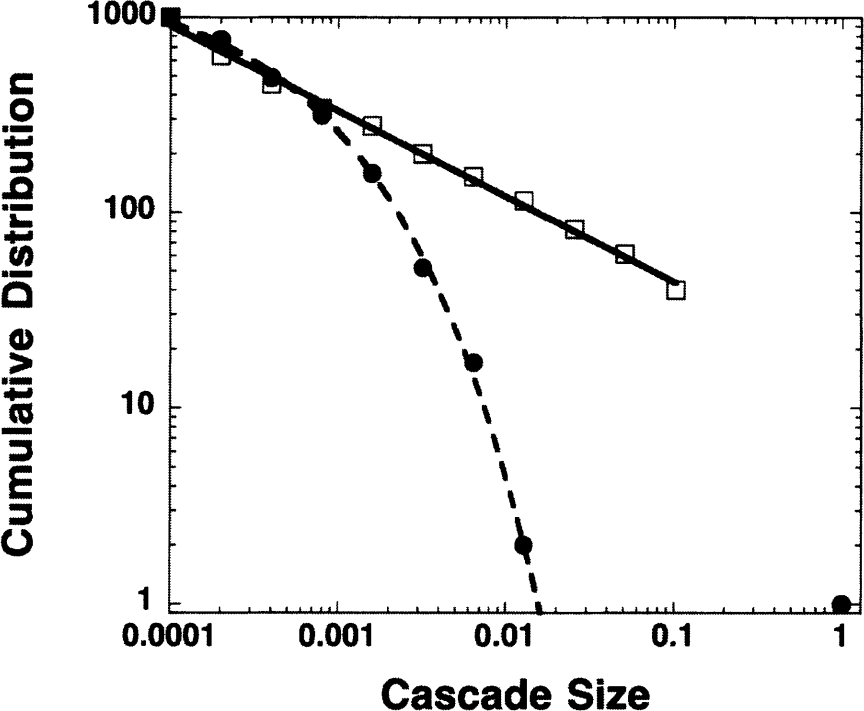
\includegraphics[width=\columnwidth]{img/cascade-size}
  \caption{Cascade Size, image from \cite{simplemodel}. $n = 1000$, squares and solid line use $z = 6.14$, circles and dashed line use $z = 1.05$.}
  \label{fig:cascade-size}
\end{figure}

Figure \ref{fig:cascade-size} shows the cumulative distribution of the cascade sizes. The size of a cascade is measured in terms of the ratio between agents in state $1$ to the total number of agents.

At the lower boundary of the cascade window, with $z = 1.05$, the curve resembels a power law distribution (note the logarithmic axes). This distribution is very similar to avalances in self-organized criticality models (TODO $wat$). This distribution can be explained by most nodes being vulnerable given the low value of $z$, so cascades can spread to neighbors very easily. The constraining factor is the connectivity of the network, that is, missing connections inhibit the cascade's progressions, not a high convincability threshold of agents.

On the other hand, the upper boundary behaves the opposite. With $z = 6.14$, the limiting factor is the large amounts of neighbors and the resulting difficulty in overcoming an individual node's threshold. Connectivity in turn is not a problem anymore, since the large amount of neighbors also gives the graph a high degree of connectivity. This leads to the distribution being very bottom-heavy, with most of the cascades failing at an early stage, since only a small amount of surrounding vulnerable agents can be convinced to switch their state. In the rare case (really just one case, see section \ref{sec:threats}) that the cascade actually manages to infect the largest vulnerable cluster, a large global cascade that converts a majority of agents is likely. This leads to a bimodal distribution, i.e. it peaks at low values, is reduced to zero in the middle and then (sort of) peaks again at large values.


\section{Threats to Validity}\label{sec:threats}

This section points out the possibly invalid points in Watts' paper\cite{simplemodel}, as well as the limitations with the model presented therein.

One limitation already mentioned in section \ref{sec:model} is that the model only allows any agent to switch its state a single time. It also lacks states beyond the binary $0$ and $1$. These make it difficult or impossible to model cascades that involve more than a single option, such as multiple competing products.

It also does not take into account relationship strength or authority. Every neighbor of a node always has the same weight and only the amount of neighbors with a certain state matters. However, this is far removed from a social network, where the persuasive power varies greatly depending on the kind of relationship between two people.

Any kind of personal knowledge or observation of a global adoption rate is not taken into account either. A cascade is always started by a single node switching its state, while in reality, several people might decide to switch without their friends directly prompting them to do so.

The bimodality mentioned in \ref{sec:findings} does not have a significant sample size. In fact, there is only a single example of a large example occurring. Calling the distribution bimodal due to a single result like that may be a stretch. Instead, more experiments should have been conducted to either rule the sample out as a fluke or confirm bimodality through more large samples appearing.

Finally, the paper itself does not have a section on threats to validity, despite it being recommended for research design\cite{yodawg}.


\bibliographystyle{abbrv}
\bibliography{paper}

\end{document}
